\documentclass{jsarticle}

% パッケージ
\usepackage[dvipdfmx]{graphicx}
\usepackage{url}
\usepackage{amsmath}
\begin{document}

% 脚注フォーマット
\renewcommand\thefootnote{\arabic{footnote})}


% 表紙

{\Large \today 提出}\\ % 提出日

\begin{center}
\vspace{120truept}
{\huge 平成28年度 卒業論文\\[10mm]
IPOほにゃらら}\\ % タイトル
\vspace{10truept}
{\Large サブタイトル}\\ % サブタイトル(なければコメントアウト)
\vspace{120truept}
{\huge 学籍番号 07-150041}\\ % 学籍番号
\vspace{50truept}
{\huge 東京大学経済学部経済学科\\[50truept]
岡部 匡志}\\ % 著者

\end{center}
\newpage
\begin{center}
{\Large IPOほにゃらら}\\ % タイトル
\end{center}

% 目次
\tableofcontents

\vspace{120truept}
% 本文
\section{はじめに\#要更新}
本稿では、日本の新規株式公開\footnote[1]{Initial Public Offering。以下、 「IPO」とする。}市場において、直近の数社のパフォーマンスがアンダープライシング\footnote[2]{\{(初値) - (公開価格)\} / (公開価格) として示される。100\%からの乖離を、初期収益率・初期乖離率と呼ぶこともある。ここで、公開価格とは、「IPO直前に希望する投資家に対して新規公開予定の株式を売却する際の価格(岡村 2011\cite{okamura})である。また、本稿では初値として、マーケットで付けられた、取引初日における最初の価格を用いる。}にどのような影響を及ぼしているのかについて考察を行う。
\section{IPOにおけるアンダープライシング}
\subsection{アノマリーとしてのアンダープライシング}
アンダープライシング自体は、国内外で一種の経済学的アノマリー\footnote[3]{例えば、辰巳・桂山 2005\cite{tatsumi}に、ファイナンス分野で知られるアノマリーが詳しい。}として知られており、表\ref{around_world}の通り、国内外でその存在が継続的に確認されている。 \par
公開価格には企業のファンダメンタルズが適切に評価されており、初値は株式市場において効率的に形成されると想定するなら、このような現象が継続的に発生しているという事実は、アノマリーと言わざるを得ない。この状況の下では、投資家は、公開価格で株式を購入し、数週間後の上場後に株式を売却するだけで、高い収益率を得られる。実際に、IPO時において、アンダーライター\footnote[4]{ここでは、株式の発行・売出しに際し、株式を売れ残った際に発行者や所有者から取得する者のことであり、日本国内においては、IPOを主導する主幹事証券会社を中心としたシンジゲート団のことを指す。}が実施する公募への抽選には個人投資家からの注文が殺到する。

\begin{table}[h]
	\caption{世界各国における初期収益率の算術平均。
	Loughran et el.(1994, updated 2015) \cite{Loughran}より一部抜粋。}
	\label{around_world}
	\centering
	\begin{tabular}{cccc}
		\hline
		国名&サンプル数&期間&平均初期収益率(100\%からの乖離) \\
		\hline \hline
		英国&4,932&1959-2012&16.0\% \\
		韓国&1,758&1980-2014& 58.8\% \\
		シンガポール&609&1973-2013&25.8\% \\
		タイ&500&1987-2012&35.1\%\\
		台湾 &1,620 &1980-2013&38.1\% \\
		中国&2,512&1990-2013&118.4\%\\
		ドイツ&736&1978-2011&24.2\% \\
		日本&3,236&1970-2013&41.7\% \\
		フランス & 697 & 1983-2010 & 10.5\% \\
		米国&12,702&1960-2012&16.9\%\\
		\hline
	\end{tabular}
\end{table}


\subsection{アンダープライシングをめぐる仮説}
アンダープライシングは、IPOにおけるアノマリー、あるいは、ある種のマーケットの歪みとして、研究者や投資家たちの強い関心を集めてきた。特に研究面の関心は、アンダープライシングを合理的に説明する決定メカニズムの解明に向けられており、現在に至るまで数多くの仮説が提案されている。\par
既存研究における、アンダープライシングの決定メカニズムをめぐる仮説は、大きく2つに分類出来るだろう。すなわち、アノマリーの原因を情報の非対称性に求めるものと、各プレーヤーの限定合理性に求めるものである。\par
前者の仮説については、岡村 2011\cite{okamura}によく整理されている。本稿では名前を列挙するに留めるが、「逆選択回避仮説(別名:Winner's Curse)」「エージェンシー仮説」「情報検事仮説」など、それぞれ、アンダーライターが公開価格を意図的に引き下げる誘引を持つことを説明している。\par

また、アンダーライターではなく、投資家の側に、公開前需要の申告\footnote[5]{日本の株式市場で実施されているブックビルディング方式における、公開価格決定プロセスの一部。}に際して、株式の市場価格の観察不能性によるリスクの存在から、公開価格を押し下げる誘引が存在することを説明した研究として、池田 (2013)\cite{ikeda}がある。\par

一方で、近年の行動経済学・行動ファイナンスの発展に伴い、プレーヤーの限定合理性を導入してアンダープライシングを説明しようとする研究が展開されている。その代表的なものとして、「後の投資家は、それまでの他の投資家が行った購入意思決定を意思決定に反映させ、自らの都合に合わせて情報を無視、あるいは軽視し、先の投資家に追随する」という、いわゆる情報カスケード効果\footnote[6]{Welch (1992)\cite{Welch}がその端緒とされている。}が挙げられるだろう。\par




現実的な解釈としては、「どの仮説が正しい/誤っている」という問題ではなく、それぞれの仮説が折り重なって実際のアンダープライシングが形成されている、ということになる。以下、本稿では、図\ref{transition}のように、アンダープライシングの程度が時期によって大きく異なっていることに注目し、情報カスケード効果を想定した、マーケット・コンディションの存在と、その解明について論じていく。

\begin{figure}[h]
  \begin{center}
  \caption{アンダープライシングの年度別平均値の推移(1997〜2016) 後述のデータより著者作成(以下同様)。}
    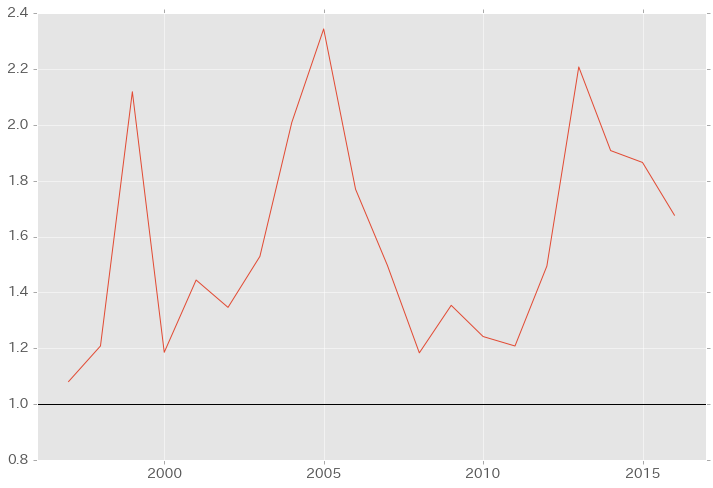
\includegraphics[clip,width=14cm]{./transition.png}
    \label{transition}
  \end{center}
\end{figure}


\section{リサーチ・デザイン}
\subsection{本研究の目的と意義\#要更新}
金子 (2009)\cite{kaneko}も指摘する通り、「間もなく発行される株式をいくら以下なら購入してもよいかを考える際に、投資家がおそらくもっとも参考にしたいと考える現在の株価が、PO(著者注:すでに株式を公開している企業が一般投資家向けに株式を発行すること)の方は存在するがIPOの方は存在しない」(p.84)ことが、IPOの初値形成における固有の事情と言える。\par
それでは、投資家は何を参考に、情報が不足する株式の購入意思決定を行っているのだろうか。\par
本稿では、直近の他のIPOにおけるパフォーマンスが、当該IPOのパフォーマンスに影響を与えると考える。すなわち、直近のIPOにおいて高いアンダープライシングが観測されたとき、投資家は自分が持つ、当該企業についてのファンダメンタルズの情報を軽視し、「今はマーケット・コンディションが良い」と考えることで、マーケットにおいて高い価格を付けるのではないか、という仮説である。\par
独自のマーケット・コンディション指数を定義し、アンダープライシングへの回帰を行った研究として、Derrien (2005)\cite{Derrien}が挙げられる。Derrienは、マーケット・コンディションを、IPO企業の属する業種インデックスの上場前3ヶ月間のパフォーマンスと定義している。本稿では、マーケット・コンディション指数を積極的に設定することはせず、当該企業のIPO時における直近の数件のIPOパフォーマンスそれ自体が、マーケット・コンディションとして機能していると考える。\par
\#要更新\#著者の知る限りにおいて、アンダープライシングを時系列的に捉えた研究は存在せず、本稿がその端緒となれば幸いである。みんな年ダミー使ってるとか、リーマン以前のデータでしかやってないこととか\par

\subsection{データ・ソース}
前章で提示した仮説を検証するために、1997年9月に上場した株式会社フォトロン(現:株式会社イマジカ・ロボット ホールディングス)から、2016年12月に上場した株式会社グッドコムアセットまでの、計1962社をサンプル・データとして用いる。\footnote[7]{データは、\url{https://github.com/M-okb/IPO_analysis}で公開している。用いたデータの内、1997年から2009年のものについては、Kaneko and Pettway’s Japanese IPO Database(\url{http://www.fbc.keio.ac.jp/~kaneko/KP-JIPO/top.htm})で公開されているデータから、2010年以降のものについては、総合投資情報サイト(\url{http://www.traders.co.jp/})、Yahoo finance(\url{http://stocks.finance.yahoo.co.jp/})から取得した。ここに感謝の意を表します。}\par
なお、上場中止・上場延期になったもの(例:株式会社ZMP)や、J-REIT(例:星野リゾート・リート投資法人)などは扱っていない。\par
\newpage

\begin{figure}[!h]
  \begin{center}
  \caption{アンダープライシング(1997〜2016)の分布ヒストグラム}
    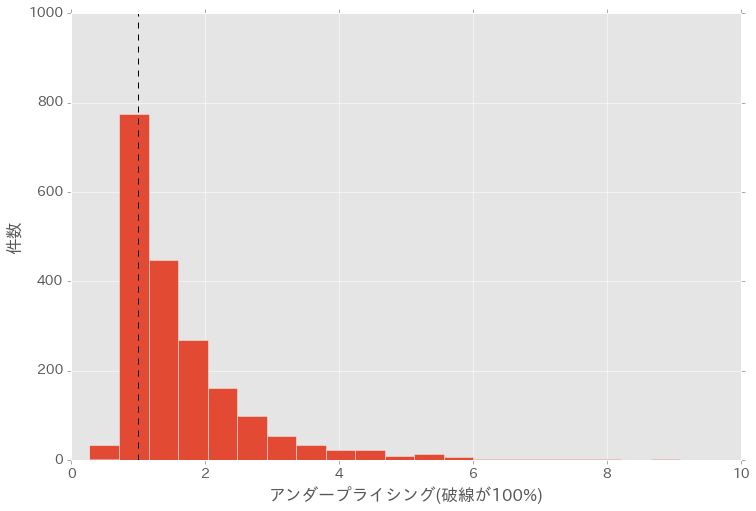
\includegraphics[clip,width=14cm]{./hist.png}
    \label{hist}
  \end{center}
\end{figure}

\begin{figure}[!h]
  \begin{center}
  \caption{アンダープライシング(1997〜2016)の対数分布ヒストグラム}
    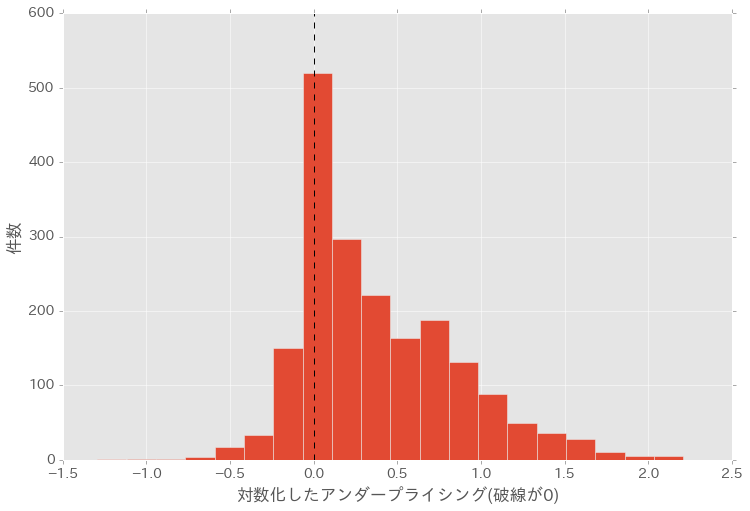
\includegraphics[clip,width=14cm]{./loghist.png}
    \label{loghist}
  \end{center}
\end{figure}

\newpage

\subsection{データの特徴}
\subsubsection{IPO件数とアンダープライシング\#要更新}
前述したとおり、図\ref{transition}のように、年度によってアンダープライシングの度合いは大きく異なる。具体的には、2000年\footnote[8]{IPOバブル崩壊の年である。政府による起業支援や、ストック・オプションの規制緩和などを受け、WEB関連銘柄を中心に市況が活性化したが、2000年3月の光通信の不正をきっかけに、WEB関連銘柄の株価は大きく値下げした。}前後で大きく下落している他、2005年がピークとなっており、2010年周辺では100\%は割らないとは言え、低迷していることが分かる。\par
全てのアンダープライシングをヒストグラムに取ったのが図\ref{hist}であり、値は正規分布せず、右に裾野の広い分布となっている。
図\ref{loghist}に、それを対数表示した。既存研究では、アンダープライシングを100分率で表示し、それを被説明変数に用いることが多かったが、本稿では100分率でなく、比率を自然対数で表示したものを用いる。\par



\begin{table}[h]
  \begin{center}
  \caption{アンダープライシングの基本統計量の5年おきの推移(1997〜2016)}
\begin{tabular*}{120mm}{@{\extracolsep{\fill}}c|ccccc}

\hline
\  & 総計 &  1997 &  2002&   2007  & 2012 \\
\hline \hline
件数 &1962 & 606 & 766 & 249 & 341 \\
\hline
標準偏差&       0.990  &0.911  &1.080 & 0.601 & 1.005 \\
\hline
平均値   &  1.647 & 1.417 & 1.836 & 1.357 & 1.840 \\
\hline
最小値    &     0.275 & 0.275 & 0.583 & 0.571&  0.531 \\
25\%tile   &       1.026 & 1.000  &1.094 & 0.941 & 1.089 \\
50\%tile    &      1.271&  1.115 & 1.472 & 1.077  &1.486 \\
75\%tile     &     1.999 & 1.500 & 2.183  &1.694 & 2.294 \\
最大値  &   9.091 & 9.091&  8.727 & 4.086 & 5.625 \\
\hline
	\end{tabular*}
	\label{stats} 
  \end{center}
\end{table}

アンダープライシングの5年おきの基本統計量の推移を表\ref{stats}に示した。どの時代でも、おおよそ、25\%tileを境目として、初期収益率がプラスとなることが分かる。\par


年度別のIPO数は図\ref{fig:year}のようになっており、多い年では、少ない年の10倍近くのIPOがある。こちらは、アンダープライシングとは異なり、IPOバブル崩壊の影響は限定的であるが、2008年のリーマン・ショックの影響を大きく受けているように見受けられる。

\#要更新\#IPO件数がアンダープライシングに与える影響についての仮説を掲載


\begin{figure}[h]
  \begin{center}
  \caption{IPO数の年度別推移(1997〜2016)}
  \begin{tabular}{c}
  \begin{minipage}{0.5\hsize}
  \begin{center}
    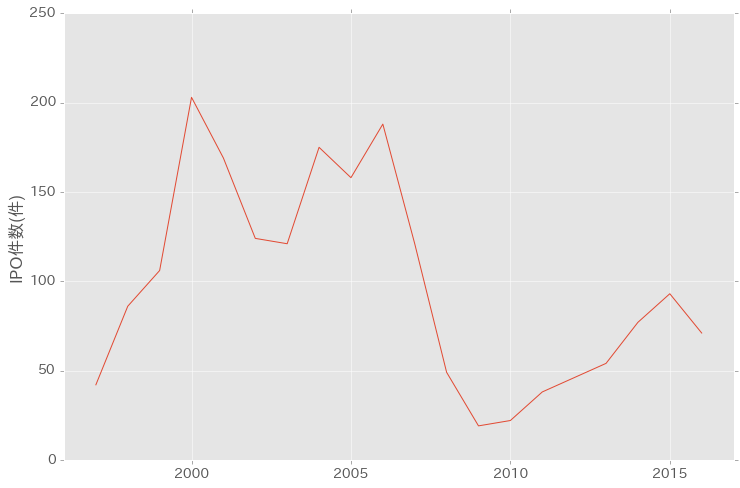
\includegraphics[clip,width=9cm]{./year_count.png}
     \end{center}
\end{minipage}
\begin{minipage}{0.5\hsize}
\begin{center}
    \label{fig:year}
\begin{tabular}{cc|cc}
		\hline
		年度 & 件数 & 年度 & 件数 \\
		\hline \hline
1997  &   42 & 2007  &  121\\
1998  &   86 & 2008   &  49\\
1999   & 106 & 2009  &   19\\
2000 &   203 & 2010  &   22\\
2001  &  169 & 2011   &  38\\
2002 &   124 & 2012  &   46\\
2003 &   121 & 2013 &    54\\
2004 &   175 & 2014   &  77\\
2005 &   158 & 2015  &   93\\
2006  &  188 & 2016 &    71\\
		\hline
	\end{tabular} 
	 \end{center}
	\end{minipage}
	  \end{tabular}
	    \end{center}
\end{figure}


\newpage

\begin{figure}[!h]
  \begin{center}
  \caption{IPO企業の上場時年齢(1997〜2016)の分布ヒストグラム}
    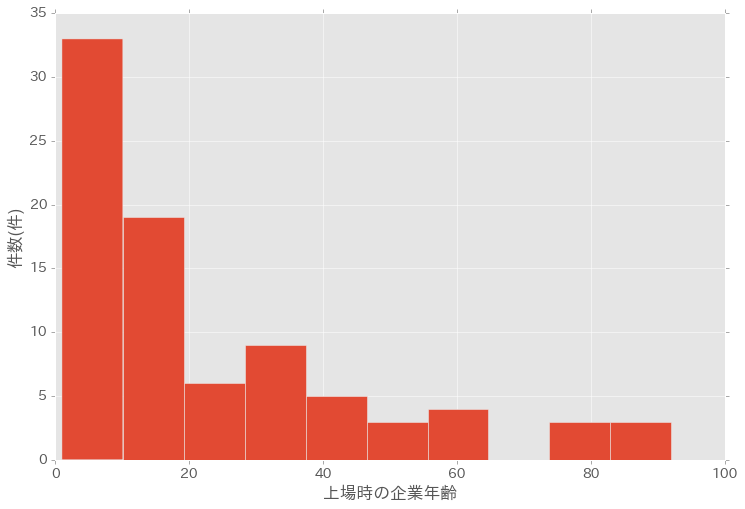
\includegraphics[clip,width=14cm]{./age.png}
    \label{agehist}
  \end{center}
\end{figure}

\begin{figure}[!h]
  \begin{center}
  \caption{IPO企業の上場時年齢の基本統計量の5年おきの推移(1997〜2016)}
\begin{tabular}{cccccc}
\hline
\  & 総計 & 1997 & 2002 & 2007 & 2012  \\
 \hline \hline
標準偏差 & 17.244 & 16.686 & 16.864 & 19.009 & 16.895   \\
\hline
平均値 & 21.724 & 24.480 & 20.295 & 23.671 & 18.613   \\
\hline
最小値 & 0 & 0 & 0 & 1 & 0   \\
25\% & 8 & 11 & 7 & 8 & 8   \\
50\% & 16 & 22 & 16 & 18 & 12   \\
75\% & 31 & 35 & 29 & 35 & 22   \\
最大値 & 96 & 95 & 91 & 96 & 89   \\
\hline
	\end{tabular}
	\label{age} 
  \end{center}
\end{figure}

\newpage

\subsubsection{上場時の企業年齢}
図\ref{agehist}と表\ref{age}に、IPO企業の、会社設立から上場までの所要年数を示した。中央値は16年と、比較的若い企業が多い。また、その構成は、年度の推移に関わらずほぼ一定であると言える。


\subsubsection{業種}
各企業は、日本証券コード委員会が定める、33業種が割り振られている。\par
業種ごとの上場企業数を示したものが表\ref{industry}である。IPOを行う企業の業種は、情報・通信業、卸売業、小売業、不動産業、サービス業などに偏っていることが分かる。

\subsubsection{主幹事証券会社}
主幹事とは、会社に代わって株式発行業務を引き受ける、幹事会社の代表のことである。公開株式の買取引受の他、ブックビルディング方式における公開価格の決定、IPOに際する社内管理体制の整備なども実施し、他のアンダーライターに比して、IPOに占める役割が大きい。日本のIPO市場では、池田 (2010)\cite{ikeda2}が指摘するように、「どの年度も主幹事を務める証券会社はわずか20社程度で、大手証券会社3社(野村、大和、日興)の主幹事シェアが高い」(p.85) 。「米国における1980から1997年までの各年で主幹事を務めた証券会社(投資銀行)数は,最大で1997年の124社(IPO件数は407件)、最小で1989年と1990年の39社(IPO件数はそれぞれ108件、110件)である」(p.85)ことを考えると、日本におけるIPO主幹事の寡占度の高さが伺える。表\ref{lead}は、今回のサンプルにおける、主幹事上位5社のシェア(案件数ベース)である。\par




主幹事証券会社がアンダープライシングに与える影響を考察した研究は、国内でも盛んであり、例えば、池田 (2010)\cite{ikeda2}や金子 (2009)\cite{kaneko}がある。
\newpage
\begin{table}[!h]
\centering

  \caption{証券コード協議会が定める33業種と本サンプルにおける件数}
\begin{tabular}{|c|c|c||c|c|c|}

\hline
番号 & 業種 & 件数 & 番号 & 業種 & 件数 \\
\hline \hline
1 & 水産・農林業 & 5 & 17 & 輸送用機器 & 15 \\
2 & 鉱業 & 3 & 18 & 精密機器 & 25 \\
3 & 建設業 & 57 & 19 & その他製品 & 51 \\
4 & 食料品 & 39 & 20 & 電気・ガス業 & 7 \\
5 & 繊維製品 & 4 & 21 & 陸運業 & 10 \\
6 & パルプ・紙 & 6 & 22 & 空運業 & 3 \\
7 & 化学 & 50 & 23 & 海運業 & 0 \\
8 & 医薬品 & 32 & 24 & 倉庫・運輸関連 & 14 \\
9 & 石油・石炭製品 & 2 & 25 & 情報・通信業 & 270 \\
10 & ゴム製品 & 1 & 26 & 卸売業 & 160 \\
11 & ガラス・土石製品 & 7 & 27 & 小売業 & 249 \\
12 & 鉄鋼 & 3 & 28 & 銀行業 & 11 \\
13 & 非鉄金属 & 9 & 29 & 証券・商品先物取引業  & 26 \\
14 & 金属製品 & 19 & 30 & 保険業 & 11 \\
15 & 機械 & 70 & 31 & その他金融業 & 26 \\
16 & 電気機器 & 96 & 32 & 不動産業 & 134 \\
17 & 輸送用機器 & 15 & 33 & サービス業 & 547 \\
18 & 精密機器 & 25 &  &  &  \\

\hline
	\end{tabular}
		\label{industry}
\end{table}

\begin{table}[h]
  \begin{center}
  \caption{主幹事上位5社のシェア(1997〜2016)}
\begin{tabular*}{120mm}{@{\extracolsep{\fill}}c|ccccc}

\hline
\ &  野村 &  大和 & 日興 & みずほ & SBI \\
\hline \hline
件数  &   536 & 399 & 293 & 74 & 35 \\
シェア & 27.3\% & 20.3\% & 14.9\% & 3.8\% & 1.8\% \\
\hline
	\end{tabular*}
	\label{lead} 
  \end{center}
\end{table}



\begin{figure}[!h]
  \begin{center}
  \caption{新興市場と非新興市場のIPO件数の推移(1997〜2016)}
    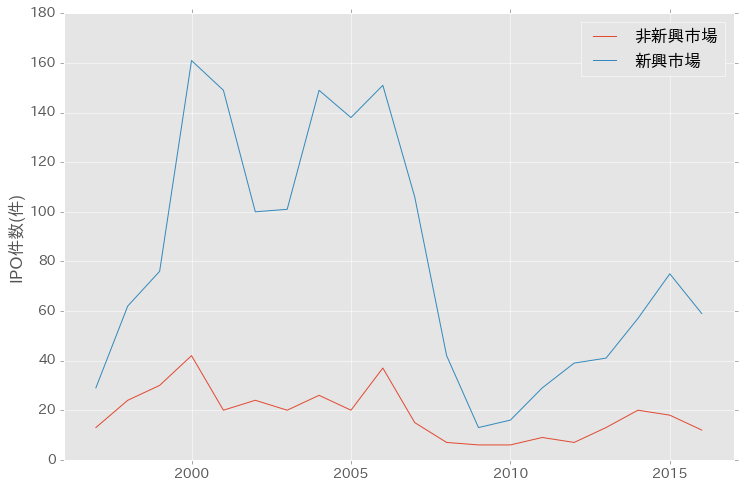
\includegraphics[clip,width=14cm]{./rising.png}
    \label{rising}
  \end{center}
\end{figure}

\newpage

\subsubsection{上場市場}

いわゆる新興市場\footnote[9]{本稿では、JASDAQ(旧店頭市場、大証ヘラクレス、NEO含む)、マザーズ、福証Q-Board、札証アンビシャス、名証セントレックス。}と、通常の市場に上場する企業の数の年度別推移を図\ref{rising}に示す。 IPO数が伸びている時期は、主に新興市場での伸びが著しいと言えよう。

\subsection{モデルの構造と想定される結果}
本稿では、「当該企業のIPOには、直近の数件のIPOのパフォーマンス自体がマーケット・コンディションとして影響している」という仮定を検証するために、アンダープライシングを被説明変数とする、p次の自己回帰モデルを用いる。パラメータは最小二乗法で推定し、AIC(赤池情報基準)から適切なラグ次数を算出する。\par
回帰式は以下のようになる。
\begin{equation}
\begin{split}
	UP_t = \alpha + \beta_u ({\rm L}) UP_t + \beta_a Age_t + \beta_{int} Interval_t + \\
	 \beta_m Market_t + \sum_{L} \beta_l Leader_t +  \sum_{I} \beta_{ind} Industry_t + \mu_t
\end{split}
\end{equation}
ここで、(L)はラグ多項式であり、$\beta_u(L) = \sum_{i=1}^p \beta_{ui} {\rm L}^i$である。\par
\#ここで$UP_t$に対してADF検定を行い、定常性(確率トレンドを持たないこと)を確認するべき?\par
\newpage
それぞれの変数について説明する。\par
\begin{description}
 \item[$UP_t$]\mbox{}\\ 
 \{(初値) - (公開価格)\} / (公開価格)の自然対数を取ったもの。
  \item[$Age_t$]\mbox{}\\
  IPO企業のIPO時における企業年齢(年)の自然対数を取ったもの。若ければ若いほど、その企業についての情報量ギャップが大きいと考えられ、負の係数が予想される。
  \item[$Interval_t$]\mbox{}\\
  前回のIPOからの日数(日)。同日にIPOが実施される場合は、片方を0とした。頻繁にIPOがあることはマーケット・コンディションが良いことと相関があると考えられるため、負の係数が予想される。
  \item[$Market_t$]\mbox{}\\
  上場市場ダミー。上場先が新興市場のとき1を、それ以外で0を取る。新興市場の方が情報量ギャップが大きいと考えられ、正の係数が予想される。
  \item[$Leader_t$]\mbox{}\\
  主幹事ダミー群。それぞれ、シェア上位5位である、野村、大和、日興、みずほ、SBIであったときに1を、それ以外で0を取る。
  \item[$Industry_t$]\mbox{}\\
  業種ダミー群。各業種のときに1を、そうでないときに0を取る。完全な多重共線性を防ぐため、サービス業ダミーの取り除いている。情報通信業や小売業などの、新しいビジネス・モデルが起こりやすい業態において、正の係数が予想される。
\end{description}\par
また、IPOのマーケット・コンディションが、上場済みの株式市場とどういった関係にあるのかを把握するために、説明変数に当該IPO時における株式マーケットのインデックス\footnote[10]{日経平均株価 【998407】・JASDAQ指数 【23337】を使用。単位はそれぞれ(円)。}を含めたモデルも推定する。その場合の回帰式は、それぞれ
\begin{equation}
\begin{split}
	UP_t = \alpha + \beta_u (L) UP_t + \beta_a Age_t + \beta_v Interval_t + \\
	 \beta_m Market_t + \sum_{K} \beta_l Leader_t +  \sum_{I} \beta_I Industry_t + \beta_n Nikkei_t+  \mu_t
\end{split}
\end{equation}

\begin{equation}
\begin{split}
	UP_t = \alpha + \beta_u (L) UP_t + \beta_a Age_t + \beta_v Interval_t + \\
	 \beta_m Market_t + \sum_{K} \beta_l Leader_t +  \sum_{I} \beta_I Industry_t + \beta_j JQ_t+  \mu_t
\end{split}
\end{equation}
となる。\par
\#インデックスも時系列データだが、$UP_t$が確率トレンドを持たないならば、見せかけの回帰は回避できている、として良いのか?\par

\newpage


\section{実証分析の結果}
\section{総括と今後の課題}

\newpage


\begin{thebibliography}{99}
\bibitem{okamura} 岡村秀夫 (2011)「IPO研究の展開」, 『商学論究, 58(3):45-65』
\bibitem{tatsumi} 辰巳憲一・桂山靖代 (2005)「IPOリターン・リバーバル —初取引日前後IPOパフォーマンスのアノマリー分析—」, 『学習院大学 経済論集, 第42巻 第3号』
\bibitem{Loughran} Loughram, T., Ritter, J. and Rydqvist, K. (1994) "Initial Public Offering: International Insights," Pacific-Basin Finance Journal 2, 165-199. (updated 2015)
\bibitem{ikeda} 池田直史 (2013) 「IPOの株価観察不能性と正の初期収益率」, 『金融経済研究, 第35号 34-51』
\bibitem{Welch} Welch, I. (1992) "Sequential Sales, Learning, and Cascades," The Journal of FINANCE 47, 695-732.
\bibitem{Derrien} Derrien, F. (2005) "IPO Pricing in "Hot" Market Conditions: Who Leaves Money On the Table?," Journal of Finance 60, 487-615
\bibitem{kaneko} 金子隆 (2009) 「IPOの過小値付け現象 −新しい解釈の試み−」, 『三田商学研究 第52巻 第2号』
\bibitem{ikeda2} 池田直史 (2010) 「IPOにおける大手証券会社の引受と初期収益率:利益相反仮説の検証」, 『三田商学研究 第53巻 第1号』
\end{thebibliography}
\end{document}